\documentclass[a4paper]{article}
\usepackage[spanish]{babel}
\usepackage[utf8]{inputenc}
\usepackage{charter}   % tipografia
\usepackage{graphicx}
%\usepackage{makeidx}
\usepackage{paralist} %itemize inline
\usepackage{pdfpages}


%\usepackage{float}
%\usepackage{amsmath, amsthm, amssymb}
%\usepackage{amsfonts}
%\usepackage{sectsty}
%\usepackage{charter}
%\usepackage{wrapfig}
%\usepackage{listings}
%\lstset{language=C}


\usepackage{color} % para snipets de codigo coloreados
\usepackage{fancybox}  % para el sbox de los snipets de codigo

\definecolor{litegrey}{gray}{0.94}

% \newenvironment{sidebar}{%
% 	\begin{Sbox}\begin{minipage}{.85\textwidth}}%
% 	{\end{minipage}\end{Sbox}%
% 		\begin{center}\setlength{\fboxsep}{6pt}%
% 		\shadowbox{\TheSbox}\end{center}}
% \newenvironment{warning}{%
% 	\begin{Sbox}\begin{minipage}{.85\textwidth}\sffamily\lite\small\RaggedRight}%
% 	{\end{minipage}\end{Sbox}%
% 		\begin{center}\setlength{\fboxsep}{6pt}%
% 		\colorbox{litegrey}{\TheSbox}\end{center}}

\newenvironment{codesnippet}{%
	\begin{Sbox}\begin{minipage}{\textwidth}\sffamily\small}%
	{\end{minipage}\end{Sbox}%
		\begin{center}%
		\vspace{-0.4cm}\colorbox{litegrey}{\TheSbox}\end{center}\vspace{0.3cm}}



\usepackage{fancyhdr}
\pagestyle{fancy}

%\renewcommand{\chaptermark}[1]{\markboth{#1}{}}
\renewcommand{\sectionmark}[1]{\markright{\thesection\ - #1}}

\fancyhf{}

\fancyhead[LO]{Sección \rightmark} % \thesection\ 
\fancyfoot[LO]{\small{Aldasoro Agustina, Bouz\'on Mar\'ia Bel\'en, Cairo Gustavo Juan}}
\fancyfoot[RO]{\thepage}
\renewcommand{\headrulewidth}{0.5pt}
\renewcommand{\footrulewidth}{0.5pt}
\setlength{\hoffset}{-0.8in}
\setlength{\textwidth}{16cm}
%\setlength{\hoffset}{-1.1cm}
%\setlength{\textwidth}{16cm}
\setlength{\headsep}{0.5cm}
\setlength{\textheight}{25cm}
\setlength{\voffset}{-0.7in}
\setlength{\headwidth}{\textwidth}
\setlength{\headheight}{13.1pt}

\renewcommand{\baselinestretch}{1.1}  % line spacing


% \setcounter{secnumdepth}{2}
\usepackage{underscore}
\usepackage{caratula}
\usepackage{url}


% ******************************************************** %
%              TEMPLATE DE INFORME ORGA2 v0.1              %
% ******************************************************** %
% ******************************************************** %
%                                                          %
% ALGUNOS PAQUETES REQUERIDOS (EN UBUNTU):                 %
% ========================================
%                                                          %
% texlive-latex-base                                       %
% texlive-latex-recommended                                %
% texlive-fonts-recommended                                %
% texlive-latex-extra?                                     %
% texlive-lang-spanish (en ubuntu 13.10)                   %
% ******************************************************** %



\begin{document}


\thispagestyle{empty}
\materia{M\'etodos Num\'ericos}
\submateria{Segundo Cuatrimestre de 2014}
\titulo{Trabajo Práctico III}
\subtitulo{Develando la mentira de los megap\'ixeles}
\integrante{Aldasoro Agustina}{86/13}{agusaldasoro@gmail.com}
\integrante{Bouz\'on Mar\'ia Bel\'en}{128/13}{belenbouzon@hotmail.com}
\integrante{Cairo Gustavo Juan}{89/13}{gjcairo@gmail.com}

\maketitle
\newpage

\thispagestyle{empty}
\vfill
\begin{abstract}
En el presente trabajo se pretende analizar y comparar distintas alternativas que pretenden dar respuesta al problema de demosaicing. Para ello, las mismas serán implementadas y sometidas a experimentación sobre fotografías crudas sintéticas \textcolor{red}{(Sinteticas quiere decir que las armamos nosotros? si no es asi, habria que ponerlo)} específicamente seleccionadas para poner de manifiesto las ventajas e inconvenientes del empleo de cada método. \\
\end{abstract}

\textbf{Palabras clave:} \\
$\bullet$ Filtro Bayer \\
$\bullet$ Demosaicing \\
$\bullet$ Interpolaci\'on \\
$\bullet$ Artifacts \\



\thispagestyle{empty}
\vspace{3cm}
\tableofcontents
\newpage


%\normalsize
\newpage

\section{Introducci\'on Te\'orica}

Promediando la década de 1990 comenzaron a introducirse al mercado las cámaras digitales de uso hogareño, empezando a sustituir desde entonces a las ampliamente difundidas cámaras de film. 
Mientras que estas últimas capturaban la imagen de forma mecánica y sin intercesión de un procesamiento digital (\textcolor{red}{¿? Asegurarse cómo es y explayarse. Estuve buscando y no entendi o no encontre nada. me parece que asi esta bien}), las cámaras electrónicas emplearon una nueva tecnología. Esta tecnolog\'ia distingue entre en el momento de obtención de un conjunto de datos cerca del objetivo – donde se obtiene una imagen que llamaremos “\textit{cruda}” – y una etapa de procesamiento automático conjunto a la reconstrucción de la imagen final. \\

En el presente trabajo nos interesará analizar un fragmento de dicha etapa conocido como \emph{demosaicing}. Para entender de qué consta, es menester comprender previamente la forma en que se capturan las imágenes al utilizar cámaras digitales.

Las cámaras digitales poseen un sensor CCD compuesto de una matriz de elementos fotosensibles, cada uno de los cuales es capaz de captar la intensidad de la luz que llega a ese punto a través de la lente. 

La tarea de capturar todos los colores reflejados por el objetivo que se quiere fotografiar no está encomendada a ninguna posición en particular, sino que cada una de ellas tiene asignada – de acuerdo a algún patrón definido  – la captura de la información perteneciente a un solo color. Cada p\'ixel de la imagen va a estar dividido en tres canales ya que la vamos a almacenar mediante RGB (Red, Green, Blue).

Ahora bien, esto genera una imagen que se aproxima a la realidad sólo en parte ya que para cada p\'ixel de la imagen tenemos la informaci\'on de s\'olo uno de sus tres canales. A causa de esto es que la misma debe ser reconstruida algorítmicamente, interpolando los valores de los colores que no fueron almacenados explícitamente para cada pixel.

En este punto nos vemos obligados a elegir un patr\'on para establecer para cada fotosensor qu\'e color va a capturar. Esta elecci\'on no es para nada trivial. Estos patrones son denominados \emph{Color Filter Array} y var\'ian de acuerdo al fabricante de c\'amaras digitales. En nuestro trabajo nos vamos a centrar en el\emph{ Filtro Bayer}, ya que es un filtro com\'unmente usado debido a que la cantidad de informaci\'on que brinda sobre el canal verde duplica a cada uno de los otros dos y el color verde es el m\'as sensible al ojo humano. 

\textcolor{blue}{*insertar imágenes por aquí y por allá*}

En este punto adquieren relevancia las diferentes propuestas de reconstrucción, entre las cuales pueden mencionarse la interpolación por asignación de valores próximos, la interpolación bilineal y interpolación direccional. Cada una de ellas admite una serie de variaciones \\

\textcolor{red}{PONEMOS ALGO sobre eso de que hay otros pasos mas para acomodar la imagen? pero que no los vamos  a hacer. a mi me parece que va kcsho}

\newpage
\section{Desarrollo}

Dada una \textit{imagen-crudo}, los valores que contiene en sus pixeles para cada canal los asumimos reales y ciertos. Por lo tanto, nos resta para cada p\'ixel averiguar sus dos canales faltantes. 

\subsection{Vecino m\'as cercano}
En este caso, para cada pixel le vamos a otorgar en sus dos canales faltantes el valor real m\'as pr\'oximo. Este m\'etodo es bastante simple algor\'itmicamente y adem\'as no tiene en cuenta dos factores: \\
\\
$\triangleright$ Por un lado, se le otorga el valor de un s\'olo pixel cercano. Esto podr\'ia representar un problema ya que existen casos donde si busco al p\'ixel de distancia m\'inima para el canal deseado la respuesta no va a ser \'unica. De este modo, nos vemos obligados a determinar qu\'e p\'ixel va a ser el elegido, pudiendo variar as\'i los valores finales acorde a la elecci\'on. \textcolor{red}{Esto fue muy fumado? o esta bien? Ponemos dibujito al respecto?} \\ 
\\
$\triangleright$ Por otro lado, al copiar el p\'ixel m\'as cercano arbitrariamente no existe ning\'un tipo de consideraci\'on sobre si es una posici\'on de un borde. \textcolor{red}{idem$\uparrow$}\\
\\
\textcolor{red}{Quedo muy corto? despues Agustin Montero nos reta..jajaj}\\

\subsection{Interpolaci\'on Bilineal}
\textcolor{blue}{Yo aca “copiar\'ia” lo del enunciado con el mismo dibujito y todo, esta mal?}
\subsection{Interpolaciones Direccionales}
\textcolor{blue}{Idem $\uparrow$}
\subsection{Algoritmo de Malvar, He y Cutler}

\newpage
\section{Resultados y discusi\'on}
\subsection{MHC}
Le da muchísima más definición/claridad a las fotos, y los bordes oscuros quedan prácticamente perfectos (comparando con bilineal, por ejemplo, aparecen colores fuertes alrededor de los bordes negros). Sigue pasando eso con los bordes blancos/mas claros, pero las zonas donde hay un salto grande entre claro y oscuro, mejora mucho.

\newpage
\section{Conclusiones y trabajo futuro}





\section{Ap\'endices}
\subsection{Ap\'endice A: Enunciado} 
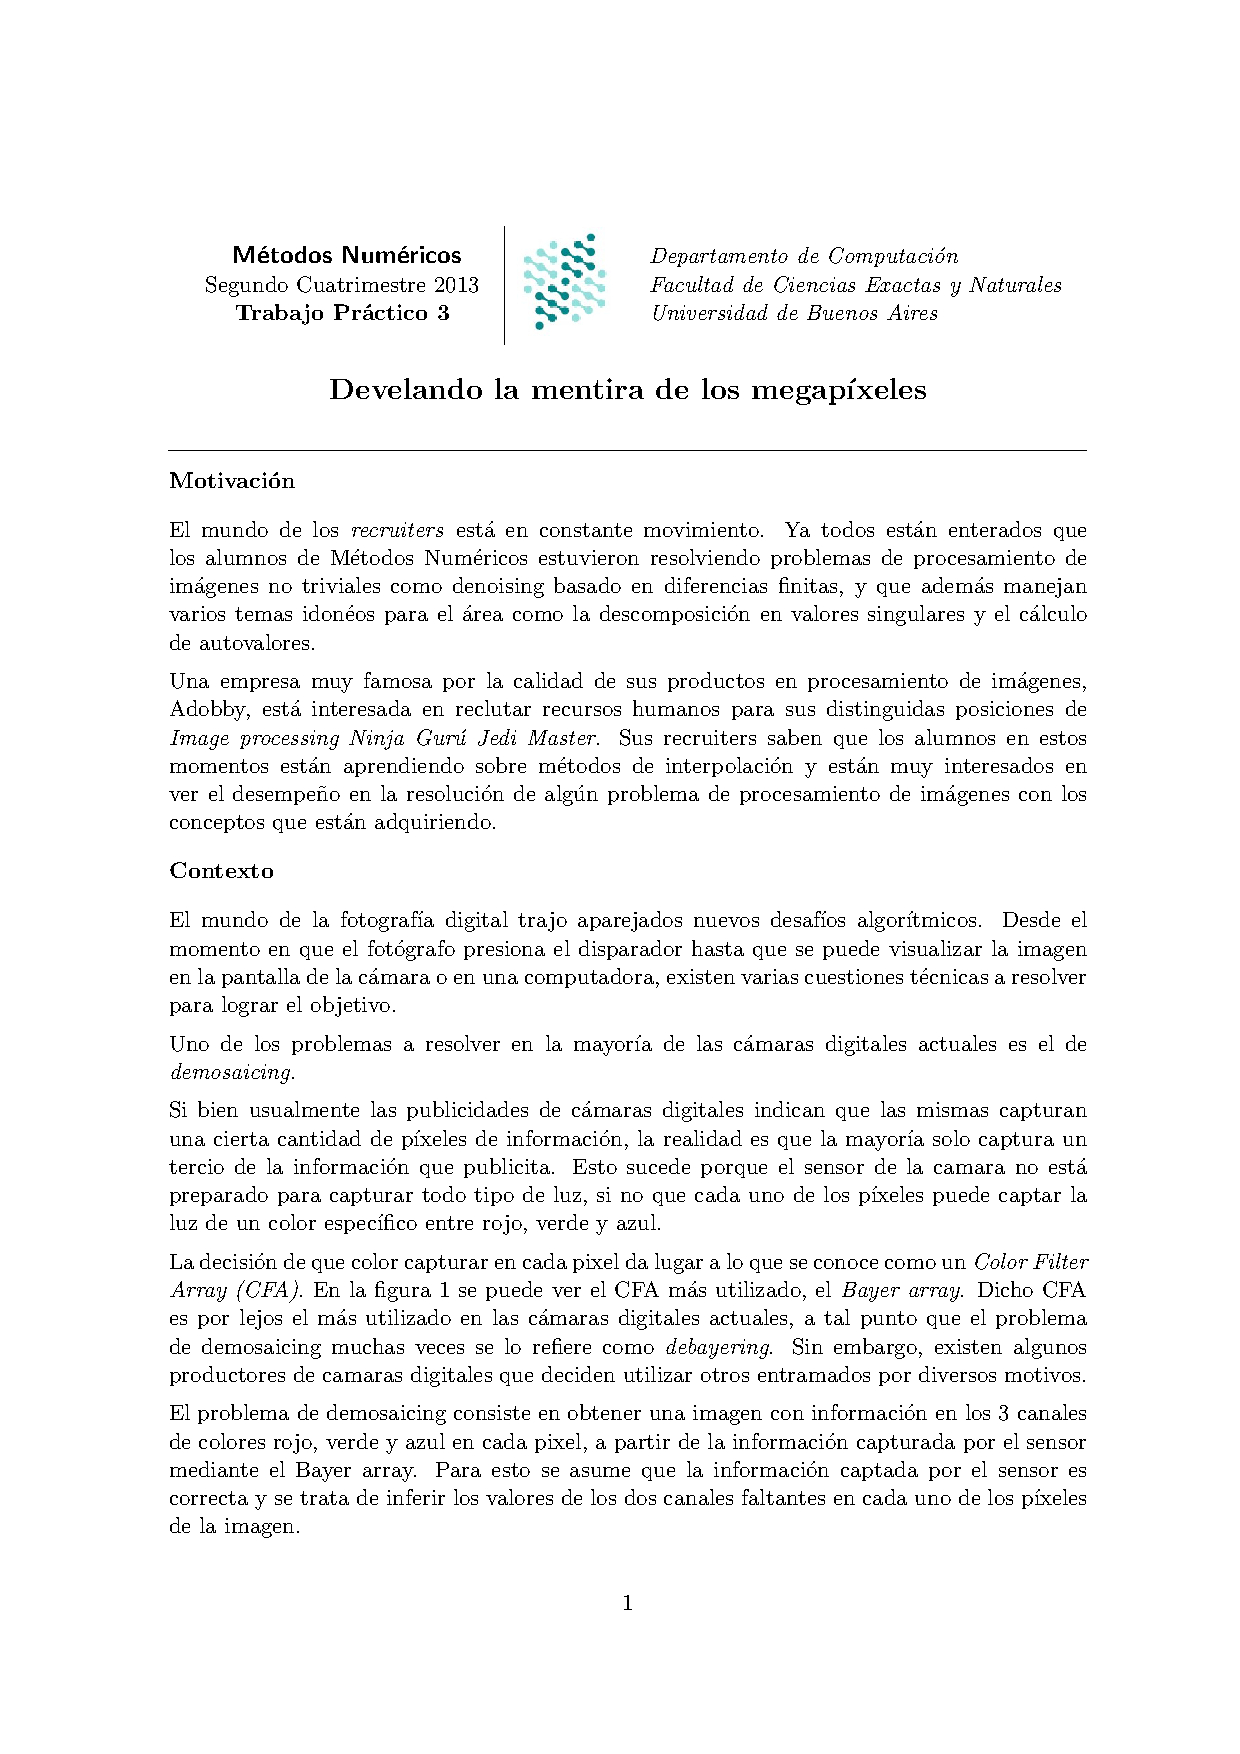
\includepdf[pages={-}]{Enunciado.pdf}

\subsection{Ap\'endice B:}
\newpage
\section{Referencias}
 
\textbf{[1]} Ron Kimmel. Demosaicing: image reconstruction from color ccd samples. \textit{IMAGE PROCESSING, IEEE TRANSACTIONS ON}, 1999. \\
\\

\textbf{[2]} Henrique S. Malvar, Li wei He, and Ross Cutler. High-quality linear interpolation for
demosaicing of bayer-patterned color images. In \textit{Proceedings of the IEEE International
Conference on Speech, Acoustics, and Signal Processing}, 2004.

\end{document}

%%%%%%%%%%%%%%%%%%%%%%%%%%%%%%%%%%%%%%%%%%%%%%%%%%%%%%%%%%%%%%%%%%%%%%%%%
\begin{figure}
  \begin{center}
	
\includegraphics[scale=0.66]{imagenes/logouba.jpg}
	\caption{Descripcion de la figura}
	\label{nombreparareferenciar}
  \end{center}
\end{figure}


\paragraph{\textbf{Titulo del parrafo} } Bla bla bla bla.
Esto se muestra en la figura~\ref{nombreparareferenciar}.



\begin{codesnippet}
\begin{verbatim}

struct Pepe {

    ...

};

\end{verbatim}
\end{codesnippet}
